\chapter{插圖}
\label{sec:graphics}

\begin{quotation}
A picture says more than a thousand words.
\begin{flushright}
--- Shakespeare
\end{flushright}
\end{quotation}

當年~Knuth~開發~\TeX~時,GIF、JPEG、PNG、EPS~等圖形格式還沒有問世,所以~DVI~不能直接支持這些格式。但是高手就是高手,Knuth~在~\TeX~上留了一個後門:\verb|\special|~命令,讓後面的~Driver~決定怎樣處理圖形。

這和當年老毛把港澳台,老鄧把釣魚島都「留給後人解決」有異曲同工之妙。曾經有位出版社的編輯看上了包老師寫的一個程序,要包老師改改當作教學輔助軟件出版,但是包老師手頭沒有~DOS~中斷的資料沒辦法加鼠標操作。該編輯說:你把鼠標驅動打包在軟件裡,讓用戶自己琢磨是怎麼回事。

下面我們會在~\ref{sec:graphics_format}~節介紹一下~\LaTeX~所用圖形格式,\ref{sec:includegraphics}~節介紹怎樣插入已有的圖形,\ref{sec:mp}--\ref{sec:pgf}~節討論怎樣製作向量圖形。

\section{圖形格式}
\label{sec:graphics_format}

\LaTeX~支持點陣圖形格式~JPEG~和~PNG,也支持向量格式~EPS~和~PDF。對於示意圖,我們應該首選向量格式;包含大量自然色彩的圖像(比如照片)應該選~JPEG,人工點陣圖像應該選~PNG。

\subsection{EPS}
80~年代中後期,PS~風頭之勁一時無兩,人們自然會考慮把它作為文檔中嵌入圖形的標準格式。然而~PS~實在太強大,人們擔心嵌入文檔的~PS~會搞破壞,於是就產生了戴著手銬的~Encapsulated PostScript(EPS)。出於同樣的原因,人們也擔心嵌入~HTML~的~ActiveX、Java Applet、JavaScript~中混入惡意代碼,所以才會對它們也有所限制。

早年間~DVI~經常被轉換為~PS,所以~EPS~就成了~\LaTeX~的標準圖形格式。

\subsection{Driver~們的口味}

\subsubsection{dvips}
\verb|dvips|~喜歡~PS,所以就愛屋及烏只支持嵌入~EPS。MiKTeX~看不慣這種壟斷行為,就把~\verb|dvips|~破解,添加了對~JPEG~和~PNG~的支持。如果你反對這種黑客破解行徑,只好找軟件把其它圖形格式轉換為~EPS。

\subsubsection{pdf\LaTeX}
pdf\LaTeX~支持~JPEG、PNG和PDF,不支持~EPS。傳說pdf\LaTeX~不支持~EPS~的原因是~PS~解釋器的版權問題。包老師認為這種說法不可信,因為~1997~年~Hàn The Thành~發佈~pdf\TeX~時~PS~已經被~PDF~趕超,Adobe~與其保護~PS~還不如保護~PDF。

\LaTeX~有兩個宏包~\verb|epstopdf|~和~\verb|pst-pdf|~可以實時地(on the fly)把~EPS~轉換為~PDF\footnote{在這裡on the fly是指在後台處理,用戶不用操心。包老師不確定把它翻譯為「實時」是否合適,因為~real time~通常被翻譯為實時。對於用戶無須干涉、知情的情況,有人說~user transparent,也有人說~black box,語言還真奇妙。}。然而前者有安全漏洞,後者用法繁瑣,用戶最好還是用其它軟件事先把~EPS~轉為~PDF。

\subsubsection{dvipdfm}
\verb|dvipdfm|~支持~JPEG、PNG、PDF,不支持~EPS,但是它可以實時地調用~Ghostscript~把~EPS~轉為~PDF。所以從圖形格式支持的角度來講,\verb|dvipdfm|~比~\verb|dvips|~和~pdf\LaTeX~都好。

那位同學說了,你這麼多廢話作甚,直接告訴我們用~\verb|dvipdfm|~不就完了。然而你別忘了~\verb|dvipdfm|~需要~DVI~作為輸入,不幸的是用來生成~DVI~的~\verb|latex|~對~JPEG~和~PNG~有意見。

綜上所述,這些~driver~都不能把圖形格式痛快地通吃,所以同學們別著急,且聽包老師慢慢忽悠怎樣轉換和處理圖形格式。

\subsection{圖形格式轉換}

注意把點陣圖形轉換為向量圖形並不能提高圖形本身的質量,正所謂「garbage in, garbage out」。

\subsubsection{JPEG~和~PNG~的範圍框}

作為中間格式的~DVI~不包含圖形本身,它只記錄圖形的尺寸和文件名,因為具體的圖形處理由後面的~driver~負責。DVI~中圖形的尺寸來自它的範圍框(bounding box),而~\verb|latex|~無法從點陣圖形文件中提取這一信息,所以我們需要以某種方式把範圍框信息告訴它。

一種方法是打開圖形文件,記下尺寸,插入圖形時加上相應的參數。

另一種方法用~\verb|ebb|~程序生成一個含範圍框信息的文件。比如下例會生成~\verb|graph.bb|~文件,有了它插入圖形時就不需要範圍框參數。注意有時此程序算出的範圍框不准,不知道是它的~bug~還是包老師的人品問題。
\begin{code}
ebb graph.jpg
\end{code}

\subsubsection{其它格式轉為EPS}
有很多程序都可以把點陣圖形轉換為~EPS,比如~\href{http://www.imagemagick.org/}{ImageMagick},以及~\href{http://www.tex.ac.uk/cgi-bin/texfaq2html?label=dvipsgraphics}{~a2ping/sam2p、bmeps、jpeg2ps、sam2p}~等。

PS~從~Level 2~開始才支持點陣圖形壓縮,所以在把其它格式轉為~EPS~時應儘量使用~Level 2~或~3,否則輸出的~EPS~會很大。

下面是一個~ImageMagick~中~\verb|convert|~程序的例子。
\begin{code}
convert photo.jpg eps2:photo.eps
\end{code}

另外還有一種~PS~虛擬打印機的方法,優點是可以把幾乎所有文件「打印」成~EPS,缺點是輸出的是~PS Level 1,即使驅動程序提供了其它~Level~的選項。

\begin{enumerate}
\item 找一個~PS~打印機驅動程序。Windows~安裝盤附帶很多打印機驅動,其中帶~PS~字樣的就是~PS~驅動。包老師選的是「HP Color LaserJet 8550-PS」,Adobe~提供的~PS~驅動效果不太好。其它驅動安裝過程可能稍有不同。
\item 安裝時端口選「FILE」,或者後面打印時選擇「Print to File」。高級選項裡的~PS~選項選「Encapsulated PostScript (EPS)」。
\item 打開點陣圖形文件,打印到上面的虛擬打印機,輸出的文件就是~EPS,但是它沒有範圍框。
\item 用~GSview~打開上面生成的~EPS,不用理會沒範圍框的警告,Options~菜單裡選上「EPS Clip」,用~File~菜單的「PS to EPS」生成含範圍框的~EPS。
\end{enumerate}

\subsubsection{其它格式轉為~PDF}

\LaTeX~附帶的~\verb|epstopdf|~程序\footnote{這個命令行程序和上面提到的~epstopdf~宏包是兩樣東西。}可以把~EPS~轉為~PDF。類似地我們也可以安裝一個~PDF~虛擬打印機,用它來把其它圖形文件轉為~PDF。

\section{插入圖形}
\label{sec:includegraphics}

\subsection{插入命令}
如今萬事俱備,只欠插入。上回講到哪兒來著?Yeah,~Knuth~的後門~\verb|\special|。

用低級命令~\verb|\special|~來插入圖形很不爽,於是~\LaTeX~v2.09~增加了~\verb|epsf|~和~\verb|psfig|~宏包。之後~\LaTeXe~推出了更好的~\verb|graphics|~和~\verb|graphicx|~宏包,這兩個宏包有個共同的命令:\verb|\includegraphics|。\verb|graphicx|~版本的語法更簡單,功能更強大,所以一般推薦用它。

插入圖形的具體命令如下,如果是點陣圖形需要加範圍框參數(左上角和右下角坐標)。

\begin{code}
\includegraphics[bb=0 0 410 307]{photo.jpg}
\end{code}

若想省略文件後綴,可在插入圖形前使用兩個命令。前者指定一個後綴列表,讓~\LaTeX~自行查找;後者告訴~\LaTeX~未知後綴的都是~EPS。
\begin{code}
\DeclareGraphicsExtensions{.eps,.mps,.pdf,.jpg,.png}
\DeclareGraphicsRule{*}{eps}{*}{}
\end{code}

\subsection{縮放、旋轉}
\Fref{tab:scale_angle}~和\Fref{tab:clip}~的選項可以用來縮放、旋轉和裁剪插圖。

\begin{table}[htbp]
\caption{includegraphics~命令的縮放和旋轉選項}
\label{tab:scale_angle}
\centering
\begin{tabularx}{350pt}{lX}
    \toprule
    scale & 縮放比例 \\
    width & 寬度 \\
    height & 高度 \\
    totalheight & 範圍框高度,旋轉時它不等於高度 \\
    keepaspectratio & 如果不使用它而同時指定插圖的寬度、高度,長寬比可能會失調;使用它時長寬比不變,寬度、高度都不超過指定參數 \\
    angle & 旋轉角度 \\
    origin & 旋轉原點 \\
    \bottomrule
\end{tabularx}
\end{table}

\begin{table}[htbp]
\caption{includegraphics~命令的裁剪選項}
\label{tab:clip}
\centering
\begin{tabularx}{350pt}{lX}
    \toprule
    viewport & 可視區域的左上角和右下角坐標。\\
    trim & 左、下、右、上四邊裁剪的數值。\\
    clip & 是否真正裁剪。預設為false,不執行裁剪,多出的部分就那樣放著;設置為true時執行裁剪。似乎是多此一舉。\\
    \bottomrule
\end{tabularx}
\end{table}

若想深入瞭解~\LaTeX~插入圖形的功能,請參考~Keith Reckdahl~的《Using Imported Graphics in \LaTeX~ and pdf\LaTeX》\citep{Reckdahl_2006}(簡稱epslatex)。

\subsection{figure環境}
插圖通常需要佔據大塊空白,所以在文字處理軟件中用戶經常需要調整插圖的位置。\LaTeX~有一個~\verb|figure|~環境可以自動完成這樣的任務,這種自動調整位置的環境稱作浮動環境。

\begin{code}
\begin{figure}[htbp]%位置選項
\centering
\includegraphics[bb=0 0 410 307,scale=.8]{photo}
\caption{10個月大的Anna}
\label{fig:anna}
\end{figure}
\end{code}

\begin{figure}[htbp]
\centering
\includegraphics[bb=0 0 410 307,scale=.8]{dscf4684}
\caption{10個月大的Anna}
\label{fig:anna}
\end{figure}

上述代碼中,\verb|[htbp]|~選項用來指定插圖排版的理想位置,這幾個字母分別代表~here、top、bottom、float page,也就是固定位置、頁頂、頁尾、單獨的浮動頁。我們可以使用這幾個字母的任意組合,一般不推薦單獨使用~\verb|[h]|,因為那個位置也許很不合適,\LaTeX~會很生氣。

\verb|\centering|~用來使插圖居中,\verb|\caption|~命令設置插圖標題,\LaTeX~會自動給浮動環境的標題加上編號。注意~\verb|label|~應放在\verb|caption|~之後,否則引用時指向的是前一個插圖。

\subsection{插入多幅圖形}
\subsubsection{並排擺放,共享標題}
當我們需要兩幅圖片並排擺放,並共享標題時,可以在~\verb|figure|~環境中使用兩個~\verb|\includegraphics|~命令。

\begin{fdemo}{
\centering
\includegraphics[scale=2]{examples/subfig_left}
\includegraphics[scale=2]{examples/subfig_right}
\captionof{figure}{反清復明}
}
\begin{figure}[htbp]
\centering
\includegraphics{left}
\includegraphics{right}
\caption{反清復明}
\end{figure}
\end{fdemo}

\subsubsection{並排擺放,各有標題}
如果想要兩幅並排的圖片各有自己的標題,可以在~\verb|figure|~環境中使用兩個~\verb|minipage|~環境,每個環境裡插入一個圖。
\begin{code}
\begin{figure}[htbp]
\centering
\begin{minipage}[t]{0.3\textwidth}
    \centering
    \includegraphics{left}
    \caption{清明}
\end{minipage}
\end{code}
\begin{code}
\begin{minipage}[t]{0.3\textwidth}
    \centering
    \includegraphics{right}
    \caption{反覆}
\end{minipage}
\end{figure}
\end{code}

\begin{figure}[htbp]
\centering
\begin{minipage}[t]{0.3\textwidth}
    \centering
    \includegraphics[scale=2]{examples/subfig_left}
    \caption{清明}
\end{minipage}
\begin{minipage}[t]{0.3\textwidth}
    \centering
    \includegraphics[scale=2]{examples/subfig_right}
    \caption{反覆}
\end{minipage}
\end{figure}

\subsubsection{並排擺放,共享標題,各有子標題}
如果想要兩幅並排的圖片共享一個標題,並各有自己的子標題,可以使用~\verb|subfig|~宏包提供的~\verb|\subfloat|~命令。

\verb|subfloat|~命令缺少寬度參數。雖然我們可以用~\verb|\hspace|~命令調整子圖的距離,子標題卻只能和子圖本身一樣寬,就會出現折行。
\begin{code}
\usepackage{subfig}
\begin{figure}[htbp]
\centering
\subfloat[清明]{
    \label{fig:subfig_a}
    \includegraphics{left}
}
\hspace{80pt}
\subfloat[反覆]{
    \label{fig:subfig_b}
    \includegraphics{right}
}
\caption{反清復明}
\end{figure}
\end{code}

每個子圖可以有各自的引用,就像這個樣子:\Fref{fig:subfig_a}、\Fref{fig:subfig_b}。
\begin{figure}[htbp]
\centering
\subfloat[清明]{
    \label{fig:subfig_a}
    \includegraphics[scale=2]{examples/subfig_left}
}
\hspace{80pt}
\subfloat[反覆]{
    \label{fig:subfig_b}
    \includegraphics[scale=2]{examples/subfig_right}
}
\caption{反清復明}
\end{figure}

\subsubsection{改進的子圖方法}
為了避免子標題折行,我們可以在~\verb|\subfloat|~裡再嵌套個~\verb|minipage|,因為後者是有寬度的。
\begin{code}
\begin{figure}[htbp]
\centering
\subfloat[清明]{
\label{fig:improved_subfig_a}
\begin{minipage}[t]{0.3\textwidth}
    \centering
    \includegraphics{left}
\end{minipage}
}
\subfloat[反覆]{
\label{fig:improved_subfig_b}
\begin{minipage}[t]{0.3\textwidth}
    \centering
    \includegraphics{right}
\end{minipage}
}
\caption{反清復明}
\end{figure}
\end{code}

\begin{figure}[htbp]
\centering
\subfloat[清明]{
\begin{minipage}[t]{0.3\textwidth}
    \centering
    \includegraphics[scale=2]{examples/subfig_left}
\end{minipage}
}
\subfloat[反覆]{
\begin{minipage}[t]{0.3\textwidth}
    \centering
    \includegraphics[scale=2]{examples/subfig_right}
\end{minipage}
}
\caption{反清復明}
\end{figure}

\section{圖形繪製工具比較}
與~\LaTeX~配套使用的繪圖工具主要有三種:\MP、PSTricks~和~PGF,它們的特點如下。

\begin{itemize}
\item 工作方式。\MP~離線繪圖,生成的~EPS~可以插入~\LaTeX~文檔;PSTricks~和~PGF~都採用在線繪圖的方式,也就是~\LaTeX~文檔內直接使用繪圖命令。
\item 兼容性。\MP~生成的~MPS~需要先轉為~PDF~才能被~pdf\LaTeX~使用;PSTricks~生成的~EPS和~pdf\LaTeX~不兼容;PGF~提供針對各種~driver~的接口,兼容性最好。
\item 功能。PSTricks~有~PS~作後盾,功能最強;\MP~擅長處理數學內容;PGF~的流程圖有獨到之處。
\end{itemize}

限於篇幅,本文只對這三種工具進行簡介。除了它們,用戶也可以考慮一些面向~\LaTeX~的繪圖前端,比如~Unix/Linux~下的~xfig~和~Windows~下的~TpX;或可以輸出~EPS~的專用軟件,比如~gnuplot~和~Matlab。

\section{\MP}
\label{sec:mp}

1989~年~John D. Hobby\footnote{Hobby 1985年從斯坦福獲博士學位,導師就是Knuth,現供職於貝爾實驗室。}開始設計一種繪圖語言及其編譯器,也就是~\MP。\MP~從~\MF~那裡獲得了大量靈感和源代碼,學生從導師那裡順點東西自然是手到擒來。\MP~和~\MF~語法類似,\MP~的主要優點在於是它輸出的是~EPS,而且支持彩色;\MF~輸出的是點陣格式,不支持彩色。Knuth~聲稱自己畫圖時只用~\MP。

從~Hobby~主頁上~\MP~的更新記錄看,它的最後版本是~0.63,年份是~1994。目前~Taco Hoekwater\footnote{他也是LuaTeX開發者之一。}繼續~\MP~的開發工作,最新版本是~1.005。

本文只對~\MP~作簡單介紹,若想深入瞭解請參閱~Hobby~的《A User's Manual for MetaPost》\citep{Hobby_2007}。

\subsection{準備工作}
用戶一般需要把~\MP~源文件(.mp)用一個命令行程序~\verb|mpost|~編譯為一種特殊的~EPS,也稱作~MPS,然後再把~MPS~插入~\LaTeX~源文件中使用。
\begin{figure}[htbp]
\centering
\begin{tikzpicture}
    \node[box] (mp) {.mp};
    \node[box, right=5 of mp] (mps) {.mps};
    \path (mp) edge [arrow] node[auto] {mpost} (mps);
\end{tikzpicture}
\caption{MetaPost~的編譯}
\label{fig:mp}
\end{figure}

一個~\MP~源文件可以包含多個圖形,一般形式如下。代碼中每行語句以~\verb|;|~結尾,註釋行以~\verb|%|~起始。每個圖形的繪圖命令包含在一對起始和結尾聲明之間。文件結尾也要有一個結尾聲明。
\begin{code}
beginfig(1); %圖形起始
...          %繪圖命令
endfig;      %圖形結尾

beginfig(2);
...
endfig;
...
end;         %文件結尾
\end{code}

假如上面的源文件名字是~\verb|fig.mp|,我們可以執行以下編譯命令。
\begin{code}
mpost fig(.mp)
\end{code}

編譯後就會生成「fig.1、fig.2、$\cdots$」~等文件,每個文件的後綴就是相應的圖形起始聲明的編號。所以此編號在一個源文件中應保持唯一,否則後生成的文件就會覆蓋前面的。

這樣的文件名管理起來很麻煩,插入它們時也不能省略後綴,因為~\LaTeX~不能識別它們。用~\verb|\DeclareGraphicsExtensions|~來逐一聲明後綴看起來很傻,自己改文件名更傻,\verb|\DeclareGraphicsRule|~也顯得不夠嚴謹。

然而~\MP~已經考慮到這個問題,為此提供了一個文件名模板命令。把下面的代碼加到源文件頭部,編譯輸出的文件名就會是「fig-01.mps、fig-02.mps、$\cdots$」。
\begin{code}
filenametemplate "%j-%2c.mps";   %加在源文件頭部
\end{code}

我們也可以把這個命令加在每個圖形的起始聲明之前,指定個性化的輸出文件名,這樣可能更便於記憶。
\begin{code}
filenametemplate "flowchart.mps" %加在每個圖形前面
\end{code}

MPS~可以用~GSview~查看,我們也可以用以下命令把它轉為~PDF~再用~Adobe Reader~查看。

\begin{code}
epstopdf flowchart.mps
\end{code}

\subsection{基本圖形對象}
為了節省空間,本節後面的示例會略去圖形起始聲明和結尾聲明等不重要的細節。

\subsubsection{直線}

繪圖命令~\verb|draw|~把幾個點以直線段連接起來。\MP~中的預設長度單位是~bp,用戶也可以使用\Fref{tab:unit}~中的其它單位。我們還可以定義一個縮放係數,把坐標都轉換成此係數的倍數,這樣以後想縮放圖形時只要改這個係數即可。

注意~\MP~中的變量賦值符號是~\verb|:=|,而~\verb|=|~用於方程式。變量在同一源文件中只須定義一次,其後的圖形中都可以使用。

\begin{fdemo}{\includegraphics{examples/line}}
draw (0,0)--(40,0)--(20,20)--(0,0);
u:=10pt; %縮放係數
draw (5u,0)--(9u,0)--(7u,2u)--cycle;
\end{fdemo}

幾段直線或曲線可以構成一條路徑(path),在路徑末尾加個~\verb|cycle|~就能構成封閉路徑(closed path)。上例中的兩個三角形看起來都是封閉的,但是前面這個其實不是真正的封閉路徑。

\subsection{點和線寬}
\verb|drawdot|~命令可以在指定坐標畫一個點,為了使它醒目些我們可以換支粗一點的畫筆。\MP~中的畫筆預設是直徑~0.5pt~的圓形,拿它畫出來的線寬就是~0.5pt。

\begin{fdemo}{\includegraphics{examples/dot}}
draw (0,0)--(10u,4u);
pickup pencircle scaled 2pt;
drawdot (0,0);
drawdot (10u,4u);
\end{fdemo}

上面的~\verb|pickup|~是一種全局操作,也就是說它會影響到之後所有的繪圖命令,我們也可以用~\verb|withpen|~為單個繪圖命令設置畫筆。

\begin{code}
draw (0,0)--(10u,4u) withpen pencircle scaled 2pt;
\end{code}

\subsubsection{曲線}
曲線和直線的命令相近,只是把連接兩個點的~\verb|--|~換成了~\verb|..|。如果共用一些坐標,直線和曲線也可以混在一條語句裡畫。

\begin{fdemo}{\includegraphics{examples/curve}}
draw (0,.5u)..(5u,3u)..(10u,1.5u)..
    (7u,0)..(5u,1.5u)..(7u,1.5u);
\end{fdemo}

\MP~的曲線用三次貝茲(Cubic B\'ezier)算法實現。用戶可以在命令中增加~direction(方向)、Tension(張力)和~Curl(曲率)等控制,限於篇幅本文不贅述。

\subsubsection{預定義圖形}
~\verb|fullcircle|~命令以原點為圓心畫一個單位圓,類似的預定義圖形還有~\verb|halfcircle、quartercircle、unitsquare|~等。注意單位正方形的參考點在左下而不在其中心。

通過不同的橫向和縱向縮放係數,我們可以把圓形和正方形變成橢圓和長方形。

\begin{code}
draw fullcircle scaled 2u;
draw halfcircle scaled 2u shifted (3u,0);
draw quartercircle scaled 2u shifted (5u,0);
draw fullcircle xscaled 4u yscaled 2u shifted (9u,0);
draw unitsquare scaled 2u shifted (12u,-u);
draw unitsquare xscaled 4u yscaled 2u shifted (15u,-u);
\end{code}

\begin{out}
\includegraphics{examples/predefined}
\end{out}

\subsection{圖形控制}

\subsubsection{線型和箭頭}
在繪製圖形時,我們不僅可以變換線寬,也可以使用多種線型。
\begin{code}
draw (0,0)--(10u,0) dashed withdots;
draw (0,1u)--(10u,1u) dashed withdots scaled 2;
draw (0,2u)--(10u,2u) dashed evenly;
draw (0,3u)--(10u,3u) dashed evenly scaled 2;
\end{code}

\begin{out}
\includegraphics{examples/dashed}
\end{out}

箭頭和直線、曲線的語法相近,注意畫反向箭頭時需要把兩個坐標用一對~\verb|()|~括起來。

\begin{fdemo}{\includegraphics{examples/arrow}}
drawarrow (0,4u)--(9u,4u);
drawarrow reverse ((0,2u)--(9u,2u));
drawdblarrow (0,0)--(9u,0);
\end{fdemo}

\subsubsection{顏色和填充}
\MP~預定義的顏色有黑、白、紅、綠、藍,它們的~RGB~值分別為(0,0,0)、(1,1,1)、(1,0,0)、(0,1,0)、(0,0,1),預設色就是黑色。

繪圖命令一般都可以通過~\verb|withcolor|~參數來使用各種顏色。封閉路徑可以用~\verb|fill|~命令填充。

\begin{fdemo}{\includegraphics{examples/color}}
draw (0,4u)--(9u,4u) withcolor red;
draw (0,2u)--(9u,2u) withcolor green;
draw (0,0)--(9u,0) withcolor blue;
\end{fdemo}

\begin{code}
fill p scaled u;
fill p scaled u shifted (3u,0) withcolor red;
fill p scaled u shifted (6u,0) withcolor green;
fill p scaled u shifted (9u,0) withcolor blue;
\end{code}

\begin{out}
\includegraphics{examples/fill}
\end{out}

另一個命令~\verb|filldraw|~可以看作是~\verb|fill+draw|,它除了填充外還會把路徑用指定的畫筆畫一遍。然而不幸的是畫邊緣和填充內部只能用同一種顏色,所以它的用處不大。

除了為每個繪圖命令單獨指定顏色,我們也可以使用一個全局命令,使得其後的繪圖命令都使用某種顏色。
\begin{code}
drawoption(withcolor blue);
\end{code}

下面的方法可以用來定義基本色以外的顏色,用基本色混色或直接用RGB值效果是一樣的。

\begin{code}
color c[];
c1 := .9red + .6green + .3blue;
c2 := (.9,.6,.3);
\end{code}

\subsubsection{圖形變換}
我們可以對路徑進行縮放、平移、旋轉等變換操作,橫向和縱向縮放可以分開進行。由於旋轉是圍繞原點進行的,所以要注意平移和旋轉的順序。下例中定義了一個~\verb|path|~變量,以便後面重用。

\begin{code}
path p;
p := (0,0)--(2,0)--(1,1.732)--cycle;
draw p scaled u;
draw p xscaled 2u yscaled u shifted (3u,0);
draw p scaled u rotated 60 shifted (8u,0);
\end{code}

\begin{out}
\includegraphics{examples/transform}
\end{out}

\subsubsection{標註}
\verb|\label|~命令可以在指定的點附近加文字標註。\MP~也可以用一對~\verb|btex|~和~\verb|etex|~來嵌入一些~\TeX~內容,比如數學標註。

\begin{code}
draw unitsquare xscaled 10u yscaled 4u;
label.top("top", (5u,4u));
label.bot("bottom", (5u,0));
label.lft("left", (0,2u));
label.rt("right", (10u,2u));
\end{code}
\begin{code}
label.ulft("upper left", (0,4u));
label.urt("upper right", (10u,4u));
label.llft("lower left", (0,0));
label.lrt("lower right", (10u,0));
label.rt(btex $E=mc^2$ etex, (3u,2u));
\end{code}

\begin{out}
\includegraphics{examples/label}
\end{out}

因為用預設方法編譯生成的~MPS~不嵌入字體,當~\MP~包含文字時,GSview~就不能正常查看。這時我們可以給編譯命令加個參數,生成的~MPS~就會包含字體信息。注意這種方法生成的~MPS~雖然~GSview~能查看,\verb|dvipdfmx|~卻不能正常處理。

\begin{code}
mpost \prologues:=2; input fig.mp
\end{code}

\subsection{編程功能}

\subsubsection{數據類型和變量}
\MP~中有10~種基本數據類型:numeric、pair、path、pen、~color~、cmykcolor、transform、string、boolean、picture。我們已經接觸過其中幾種,比如縮放係數~u~就是一個~numeric,一個點的坐標是一個~pair,幾個點用直線或曲線連起來是一個~path,pencircle~是一種~pen,black~是一種~color,scaled、rotated、shifted~都是~transform。

numeric~類型變量的精度是~1/65536,它的絕對值不能超過~4096,在計算過程中數值可以達到~32768。這樣的規定也應歸功於當年的電腦硬件,不過對於科技文檔插圖而言,4096~一般還是夠用的。

除了預設的~numeric,其它變量在使用之前都需要用數據類型來顯式聲明。相同類型的變量可以在一行語句中聲明,但是帶下標的變量不能放在同一行(這個規定很蹊蹺)。
\begin{code}
numeric x,y,z;    %正確
numeric x1,x2,x3; %錯誤
numeric x[];      %正確
\end{code}

\subsubsection{數學運算}
\MP~中可以使用普通的運算符,比如~\verb|+ - * /|;也提供一些特殊的運算符,比如~\verb|a++b|~表示$\sqrt{a^2+b^2}$,\verb|a+-+b|~表示$\sqrt{a^2-b^2}$;另外\Fref{tab:math_function}~列出一些常用數學函數。

\begin{table}[htbp]
\caption{數學函數}
\label{tab:math_function}
\centering
\begin{tabular}{llll}
    \toprule
    abs     & 絕對值   & mexp & 指數 \\
    round   & 四捨五入 & mlog & 對數 \\
    ceiling & 向上圓整 & sind & 正弦 \\
    floor   & 向下圓整 & cosd & 餘弦 \\
    mod     & 模余     & normaldeviate & 正態分佈隨機數 \\
    sqrt    & 開方     & uniformdeviate & 均勻分佈隨機數 \\
    \bottomrule
\end{tabular}
\end{table}

\subsubsection{循環}
當執行重複任務時,循環語句可以讓程序變得簡潔。注意下例中的循環語句是一條命令,之所以分成三行寫是為了看起來清晰點。

\begin{fdemo}{\includegraphics{examples/loop}}
draw (0,0) %注意這裡沒有分號
for x=1 upto 3: 
    ..(x*x,x)*u 
endfor;
\end{fdemo}

循環語句預設步長是~1,我們也可以改用其它步長。\verb|upto|~其實就是~\verb|step 1 until|~的縮寫方式。
\begin{code}
for x=1 step .5 until 3: 
\end{code}

\section{PSTricks}
\label{sec:pstricks}

PSTricks~是一個基於~PS~的宏包,有了它用戶就可以直接在~\LaTeX~文檔中插入繪圖命令。PSTricks~早期的作者是~Timothy Van Zandt\footnote{法國Insead大學經濟系教授。},初始開發年月不詳,他於~1997~年退居二線,之後由~Denis Girou、Sebastian Rahtz\footnote{牛津大學計算機系網管。}、Herbert Voß~等維護。

本文只介紹~PSTricks~的基本功能,若想深入瞭解請參閱~Van Zandt~的《PSTricks User's Guide》\citep{Zandt_2007}。另外\Fref{tab:pst_add}~列出了一些可以和~PsTricks~配合使用的輔助宏包。

\begin{table}[htbp]
\caption{PSTricks~輔助宏包}
\label{tab:pst_add}
\centering
\begin{tabular}{llll}
    \toprule
    multido & 循環語句    & pst-eucl & 幾何函數 \\    
    pst-plot & 函數繪圖   & pst-math & 弧度三角函數 \\
    pst-plot3d & 三維繪圖 & pstricks-add & 極坐標 \\  
    \bottomrule
\end{tabular}
\end{table}

\subsection{準備工作}
首先要引入~PSTricks~宏包。PSTricks~中預設長度單位是~1cm,我們也可以設置自己的單位。
\psset{unit=10pt}
\begin{code}
\usepackage{pstricks}
\psset{unit=10pt}
\end{code}

繪圖命令一般要放在~\verb|pspicture|~環境裡,這樣~\LaTeX~就會給圖形預留一個矩形區域,注意這個矩形要能容納所有圖形對象。為了節省空間,在本節後面的示例代碼中,~\verb|pspicture|~環境將被略去。

\begin{code}
\begin{pspicture}(0,0)(4,2)
...
\end{pspicture}
\end{code}

另外需要注意的是,嵌入~\LaTeX~的~PSTricks~生成的是~PS,\verb|dvips|~可以處理,\verb|dvipdfm|~和pdf\LaTeX~則不能。所以如果使用後兩種~driver,需要先行生成~EPS。

第一種方法是把~PSTricks~代碼放進一個空白的\LaTeX~頁面,用它生成一個簡單的~DVI。

\begin{code}
\documentclass{article}
\usepackage{pstricks}
\pagestyle{empty}   %頁面樣式為空

\begin{document}
\psset{unit=10pt}
\colorbox{white}{%
    \begin{pspicture}(0,0)(4,2)%
    \psdot(0,0)%
    \psdots(0,2)(2,2)(4,2)%
    \end{pspicture}%
}
\end{document}
\end{code}

然後用以下命令把~DVI~轉為~EPS,\verb|-E|~參數即代表~EPS。上面代碼中的~colorbox~使得生成的~EPS~有正確的範圍框。

\begin{code}
dvips pst_dots(.dvi) -E -o dots.eps
\end{code}

第二種方法是用~\verb|pst-eps|~宏包,它能夠在線處理~PSTricks~代碼並生成~EPS,這樣用戶就可以在同一文件中使用該~EPS。

然而~\verb|dvipdfmx|~不能正確處理~\verb|pst-eps|~生成的~EPS。它和~\verb|\rput|、\verb|\uput|~命令,\verb|pst-plot|~宏包中的~\verb|\psaxes|~命令都不兼容。類似的~\verb|ps4pdf|~宏包和~\verb|tabularx|~宏包不兼容。

\begin{comment}
\usepackage{pst-eps}
\PSTtoEPS[bbllx=0,bblly=0,bburx=4,bbury=2,makeeps=all]
{dots.eps}{
    \psdot(0,0)
    \psdots(0,2)(2,2)(4,2)
}
\includegraphics{dots.eps}
\end{comment}

\subsection{基本圖形對象}
\subsubsection{點}
我們可以用以下命令畫一個或多個點。
\begin{comment}
\PSTtoEPS[bbllx=0,bblly=0,bburx=4,bbury=2,makeeps=all]
{examples/dot.eps}{
    \psdot(0,0)
    \psdots(0,2)(2,2)(4,2)
}
\end{comment}

\begin{fdemo}{\includegraphics{examples/pst_dot.eps}}
\psdot(0,0)
\psdots(0,2)(2,2)(4,2)
\end{fdemo}

\subsubsection{直線、多邊形、矩形}
\verb|\psline|~命令把多個點用直線段連接起來,線段之間的連接預設為尖角,也可以設置圓角。
\begin{comment}
\PSTtoEPS[bbllx=0,bblly=0,bburx=9,bbury=2,makeeps=all]
{examples/line.eps}{
    \psline(0,0)(2,2)(4,0)
    \psline[linearc=.3](5,0)(7,2)(9,0)
}
\end{comment}

\begin{fdemo}{\includegraphics{examples/pst_line.eps}}
\psline(0,0)(2,2)(4,0)
\psline[linearc=.3](5,0)(7,2)(9,0)
\end{fdemo}

\verb|\pspolygon|~命令和~\verb|\psline|~類似,但是它會形成封閉路徑。
\begin{comment}
\PSTtoEPS[bbllx=0,bblly=0,bburx=9,bbury=2,makeeps=all]
{examples/polygon.eps}{
    \pspolygon(0,0)(2,2)(4,0)
    \pspolygon[linearc=.3](5,0)(7,2)(9,0)
}
\end{comment}

\begin{fdemo}{\includegraphics{examples/pst_polygon.eps}}
\pspolygon(0,0)(2,2)(4,0)
\pspolygon[linearc=.3](5,0)(7,2)(9,0)
\end{fdemo}

矩形用~\verb|\psframe|~命令,其參數就是矩形左下角和右上角的坐標。矩形也可以設置圓角。
\begin{comment}
\PSTtoEPS[bbllx=0,bblly=0,bburx=9,bbury=2,makeeps=all]
{examples/frame.eps}{
    \psframe(0,0)(4,2)
    \psframe[framearc=.3](5,0)(9,2)
}
\end{comment}

\begin{fdemo}{\includegraphics{examples/pst_frame.eps}}
\psframe(0,0)(4,2)
\psframe[framearc=.3](5,0)(9,2)
\end{fdemo}

\subsubsection{圓、橢圓、圓弧、扇形}
圓形用~\verb|\pscircle|~命令,參數是圓心和半徑。橢圓用~\verb|\psellipse|~命令,參數是中心、長徑、短徑。注意這兩個命令的半徑參數用不同的括號,可能是作者的筆誤。
\begin{comment}
\PSTtoEPS[bbllx=0,bblly=0,bburx=7,bbury=2,makeeps=all]
{examples/circle.eps}{
    \pscircle(1,1){1}
    \psellipse(5,1)(2,1)
}
\end{comment}

\begin{fdemo}{\includegraphics{examples/pst_circle.eps}}
\pscircle(1,1){1}
\psellipse(5,1)(2,1)
\end{fdemo}

圓弧用~\verb|\psarc|~命令,其參數是圓心、半徑、起止角度,逆時針作圖。~\verb|\psarcn|~類似,只是順時針作圖。扇形用~\verb|\pswedge|~命令。
\begin{comment}
\PSTtoEPS[bbllx=0,bblly=0,bburx=11,bbury=2,makeeps=all]
{examples/arc.eps}{
    \psarc(1,0){2}{0}{120}
    \psarcn(5,0){2}{120}{0}
    \pswedge(9,0){2}{0}{120}
}
\end{comment}

\begin{fdemo}{\includegraphics{examples/pst_arc.eps}}
\psarc(1,0){2}{0}{120}
\psarcn(5,0){2}{120}{0}
\pswedge(9,0){2}{0}{120}
\end{fdemo}

\subsubsection{曲線}
\verb|\pscurve|~命令把一系列點用平滑曲線連接起來;它的變形版本~\verb|\psecurve|~命令不顯示曲線的兩個端點;另一變形命令~\verb|\psccurve|~則把曲線封閉起來。

參數~\verb|showpoints=true|~用來顯示曲線的構成點,此參數也可用於其它繪圖命令。
\begin{comment}
\PSTtoEPS[bbllx=0,bblly=0,bburx=15,bbury=2,makeeps=all]
{examples/curve.eps}{
    \pscurve[showpoints=true](0,1)(1,2)(3,0)(4,2)(1,0)
    \psecurve[showpoints=true](5,1)(6,2)(8,0)(9,2)(5,0)
    \psccurve[showpoints=true](11,1)(12,2)(14,0)(15,2)(12,0)
}
\end{comment}

\begin{code}
\pscurve[showpoints=true](0,1)(1,2)(3,0)(4,2)(1,0)
\psecurve[showpoints=true](5,1)(6,2)(8,0)(9,2)(5,0)
\psccurve[showpoints=true](11,1)(12,2)(14,0)(15,2)(12,0)
\end{code}
\begin{out}
\includegraphics{examples/pst_curve.eps}
\end{out}

\verb|\psbezier|~命令輸出一條貝茲曲線,其參數就是曲線的控制點。
\begin{comment}
\PSTtoEPS[bbllx=0,bblly=0,bburx=6,bbury=2,makeeps=all]
{examples/bezier.eps}{
    \psbezier[showpoints=true]
        (0,0)(2,2)(4,0)(6,2)
}
\end{comment}

\begin{fdemo}{\includegraphics{examples/pst_bezier.eps}}
\psbezier[showpoints=true]
    (0,0)(2,2)(4,0)(6,2)
\end{fdemo}

拋物線用~\verb|\psparabola|~命令,它有兩個參數,第一個是拋物線通過的一點,第二個是拋物線的頂點。
\begin{comment}
\PSTtoEPS[bbllx=0,bblly=0,bburx=2,bbury=2,makeeps=all]
{examples/parabola.eps}{
    \psparabola[showpoints=true]
        (2,2)(1,0)
}
\end{comment}

\begin{fdemo}{\includegraphics{examples/pst_parabola.eps}}
\psparabola[showpoints=true]
    (2,2)(1,0)
\end{fdemo}

\subsubsection{網格和坐標}
科技製圖通常會用到坐標網格。\verb|\psgrid|~命令輸出一個矩形網格,它有三個參數點。網格坐標標註在通過第一個點的兩條直線上,第二和第三個點是矩形的兩個對角頂點。當第一個參數省略時,坐標標註在通過第一個頂點的兩條矩形邊上。
\begin{comment}
\psset{unit=10pt}
\PSTtoEPS[bbllx=-1,bblly=-1,bburx=8.4,bbury=2.4,makeeps=all]
{examples/grid.eps}{
    \psgrid(0,0)(-1,-1)(3,2)
    \psgrid(5,0)(8,2)
}
\end{comment}

\begin{code}
\psgrid(0,0)(-1,-1)(3,2)
\psgrid(5,0)(8,2)
\end{code}
\begin{out}
\includegraphics{examples/pst_grid.eps}
\end{out}

\verb|pst-plot|~宏包提供的~\verb|\psaxes|~命令輸出坐標軸。它的參數和~\verb|\psgrid|~的類似,刻度和標註都可以靈活地設置,也可以把坐標軸改成一個矩形框的形式。
\begin{code}
\psset{unit=10pt}
\psaxes{<->}(0,0)(-1,-1)(3,2)
\psaxes[tickstyle=top,labels=none]{->}(5,0)(8,2)
\psaxes[axesstyle=frame,tickstyle=top]{->}(10,0)(13,2)
\end{code}
\begin{out}
\includegraphics{examples/pst_axis.eps}
\end{out}

\subsection{圖形控制}
\subsubsection{線型和箭頭}
PSTricks~中的預設線寬是~0.8pt,預設線型是實線。以下參數可以控制單個繪圖命令的線寬和線型。
\begin{comment}
\psset{unit=10pt}
\PSTtoEPS[bbllx=0,bblly=0,bburx=9,bbury=4,makeeps=all]
{examples/linestyle.eps}{
    \psline[linewidth=1.5pt](0,4)(9,4)
    \psline[linestyle=dotted](0,2)(9,2)
    \psline[linestyle=dashed](0,0)(9,0)
}
\end{comment}

\begin{fdemo}{\includegraphics{examples/pst_linestyle.eps}}
\psline[linewidth=1.5pt](0,4)(9,4)
\psline[linestyle=dotted](0,2)(9,2)
\psline[linestyle=dashed](0,0)(9,0)
\end{fdemo}

我們也可以用命令~\verb|\psset|~命令來設置全局參數。
\begin{code}
\psset{linewidth=1pt,linestyle=dashed}
\end{code}

以下參數可以控制繪圖命令的箭頭。
\begin{comment}
\PSTtoEPS[bbllx=0,bblly=0,bburx=9,bbury=4,makeeps=all]
{examples/arrow.eps}{
    \psline{->}(0,4)(9,4)
    \psline{<-}(0,2)(9,2)
    \psline{<->}(0,0)(9,0)
}
\end{comment}

\begin{fdemo}{\includegraphics{examples/pst_arrow.eps}}
\psline{->}(0,4)(9,4)
\psline{<-}(0,2)(9,2)
\psline{<->}(0,0)(9,0)
\end{fdemo}

\subsubsection{顏色和填充}
PSTricks~預定義的顏色有~black、darkgray、gray、lightgray、white~等灰度顏色,也有~red、green、blue、cyan、magenta、yellow~等彩色。我們也可以自定義灰度顏色和彩色。

\begin{code}
\newgray{mygray}{.3}
\newrgbcolor{mycolor}{.3 .4 .5}
\end{code}

以下參數可以控制單個繪圖命令的顏色,我們也可以用~\verb|\psset|~命令設置全局參數。
\begin{comment}
\PSTtoEPS[bbllx=0,bblly=0,bburx=9,bbury=4,makeeps=all]
{examples/color.eps}{
    \psline[linecolor=red](0,4)(9,4)
    \psline[linecolor=green](0,2)(9,2)
    \psline[linecolor=blue](0,0)(9,0)
}
\end{comment}

\begin{fdemo}{\includegraphics{examples/pst_color.eps}}
\psline[linecolor=red](0,4)(9,4)
\psline[linecolor=green](0,2)(9,2)
\psline[linecolor=blue](0,0)(9,0)
\end{fdemo}

以下參數可以控制單個繪圖命令的填充模式和填充顏色,注意只有封閉路徑才可以填充。
\begin{comment}
\PSTtoEPS[bbllx=0,bblly=0,bburx=11,bbury=2,makeeps=all]
{examples/fill.eps}{
    \pscircle[fillstyle=solid,fillcolor=red](1,1){1}
    \pscircle[fillstyle=vlines](4,1){1}
    \pscircle[fillstyle=hlines](7,1){1}
    \pscircle[fillstyle=crosshatch](10,1){1}
}
\end{comment}

\begin{code}
\pscircle[fillstyle=solid,fillcolor=red](1,1){1}
\pscircle[fillstyle=vlines](4,1){1}
\pscircle[fillstyle=hlines](7,1){1}
\pscircle[fillstyle=crosshatch](10,1){1}
\end{code}
\begin{out}
\includegraphics{examples/pst_fill.eps}
\end{out}

\subsection{對象佈局}
\subsubsection{平移}
參數~\verb|origin|~可以讓一個圖形對象平移到指定的坐標點,我們也可以用~\verb|\psset|~命令設置全局平移參數。
\begin{comment}
\PSTtoEPS[bbllx=0,bblly=0,bburx=7,bbury=2,makeeps=all]
{examples/origin.eps}{
    \psframe(0,0)(3,2)
    \psframe[origin={4,0}](0,0)(3,2)
}
\end{comment}

\begin{fdemo}{\includegraphics{examples/pst_origin.eps}}
\psframe(0,0)(3,2)
\psframe[origin={4,0}](0,0)(3,2)
\end{fdemo}

\subsubsection{旋轉}
\verb|\rput|~命令可以對一個圖形對象同時進行旋轉和平移操作。它有兩個參數,第一個是旋轉角度,第二個是平移到的坐標點。
\begin{fdemo}{\includegraphics{examples/pst_rput.eps}}
\psframe(0,0)(3,2)
\rput{30}(5,0){\psframe(0,0)(3,2)}
\end{fdemo}

\subsubsection{文字標註}
\verb|\rput|~命令還可以在指定的坐標點標註文字,這時它的第一個參數是坐標點相對於標註的位置。其取值可以是縱向的~t、b(上下),或橫向的~l、r(左右),也可以是縱向和橫向位置的組合。
\begin{fdemo}{\includegraphics{examples/pst_label.eps}}
\pspolygon(0,0)(4,0)(2,3)
\rput[r](0,0){A}
\rput[l](4,0){B}
\rput[b](2,3){C}
\end{fdemo}

\verb|\rput|~生成的標註就在坐標點上,有時會感覺離圖形太近。另一個命令~\verb|\uput|~則生成預設距離指定坐標點~5pt的標註,它的第一個參數是標註相對於坐標點的角度。
\begin{fdemo}{\includegraphics{examples/pst_uput.eps}}
\pspolygon(0,0)(4,0)(2,3)
\uput[l](0,0){A}
\uput[r](4,0){B}
\uput[u](2,3){C}
\end{fdemo}

\verb|\uput|~的角度參數可以是任意角度,也可以是字母,參見。注意~\verb|\uput|~的角度參數和~\verb|\rput|~命令的參考點位置參數的定義幾乎正好相反,這也許反映了作者灑脫的風格。

\begin{table}[htbp]
\caption{uput~命令的角度參數}
\label{tab:uput}
\centering
\begin{tabular}{lrlr}
    \toprule
    r &   0$^\circ$ & ur &  45$^\circ$ \\
    u &  90$^\circ$ & ul & 135$^\circ$ \\
    l & 180$^\circ$ & dl & 225$^\circ$ \\
    d & 270$^\circ$ & dr & 315$^\circ$ \\
    \bottomrule
\end{tabular}
\end{table}

\section{PGF}
\label{sec:pgf}
PGF~和~Beamer~的作者都是~Till Tantau\footnote{德國Lübeck大學計算機研究所教授。}。Tantau~當初開發~Beamer~是為了應付~2003~年他的博士學位論文答辯,之後它在~CTAN~上流行開來。2005~年~PGF~從~Beamer~項目中分離出來,成為一個獨立的宏包。

本文只對~PGF~作簡單介紹,若想深入瞭解請參閱~Tantau~的《TikZ and PGF Manual》\citep{Tantau_2008}。

\subsection{準備工作}
一般人們並不直接使用~PGF~命令,而是通過它前端~TikZ~來調用~PGF。在引用~\verb|tikz|~宏包之前,用戶需要設置~PGF~系統~driver。
\begin{code}
\def\pgfsysdriver{pgfsys-dvipdfmx.def}
\usepackage{tikz}
\end{code}

PGF~的預設長度單位是~1cm,我們也可以改用其它單位。注意這樣預定義的長度單位有時會失效,這可能是~PGF~的~bug。
\begin{code}
\pgfsetxvec{\pgfpoint{10pt}{0}}
\pgfsetyvec{\pgfpoint{0}{10pt}}
\end{code}

TikZ~提供一個~\verb|tikz|~命令和一個~\verb|tikzpicture|~環境,具體繪圖指令可以放在~\verb|tikz|~後面,也可以放在~\verb|tikzpicture|~中間。兩種方法效果相同,用戶可以任意選擇。為了節省空間,本節的示例將省略部分環境代碼。
\begin{code}
\tikz ...   %繪圖命令
\begin{tikzpicture}
...         %繪圖命令
\end{tikzpicture}
\end{code}

\subsection{基本圖形對象}
\subsubsection{直線、多邊形、矩形}
TikZ~中直線的語法和~\MP~類似,加~\verb|cycle|~參數才能構成真正的封閉路徑。
\begin{fdemo}{
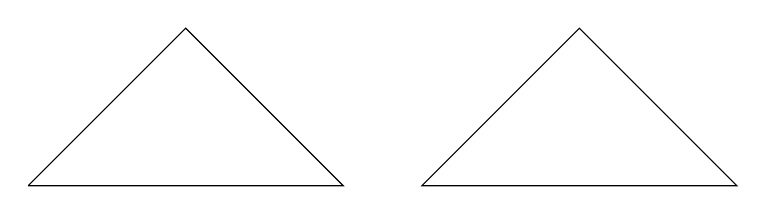
\begin{tikzpicture}
\draw (0,0)--(4,0)--(2,2)--(0,0);
\draw (5,0)--(9,0)--(7,2)--cycle;
\end{tikzpicture}
}
\draw (0,0)--(4,0)--(2,3)--(0,0);
\draw (5,0)--(9,0)--(7,3)--cycle;
\end{fdemo}

矩形命令如下,它的兩個參數是矩形的兩個對角頂點。
\begin{fdemo}{
\begin{tikzpicture}
\draw (0,0) rectangle (4,2);
\end{tikzpicture}
}
\draw (0,0) rectangle (4,2);
\end{fdemo}

\subsubsection{圓、橢圓、弧}
圓和橢圓命令如下,圓的參數是圓心和半徑,橢圓的參數是中心、長徑、短徑。
\begin{fdemo}{
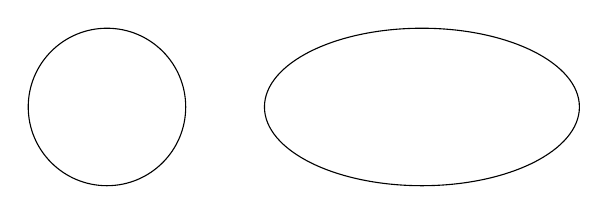
\begin{tikzpicture}
\draw (1,1) circle (1);
\draw (5,1) ellipse (2 and 1);
\end{tikzpicture}
}
\draw (1,1) circle (1);
\draw (5,1) ellipse (2 and 1);
\end{fdemo}

圓弧和橢圓弧命令如下,圓弧的參數是起始點,起始角度、終止角度、半徑;橢圓弧則把半徑換成了長徑和短徑。
\begin{fdemo}{
\begin{tikzpicture}
\draw (2,1) arc (0:270:1);
\draw (7,1) arc (0:270:2 and 1);
\end{tikzpicture}
}
\draw (2,1) arc (0:270:1);
\draw (7,1) arc (0:270:2 and 1);
\end{fdemo}

\subsubsection{曲線和拋物線}
曲線命令如下,中間的參數是控制點。
\begin{fdemo}{
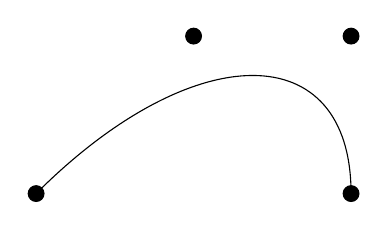
\begin{tikzpicture}
\draw (0,0) .. controls (2,2) 
    and (4,2) .. (4,0);
\filldraw (0,0) circle (.1)
    (2,2) circle (.1)
    (4,2) circle (.1)
    (4,0) circle (.1);
\end{tikzpicture}
}
\draw (0,0) .. controls (2,2) 
    and (4,2) .. (4,0);
\end{fdemo}

拋物線命令如下,除了起止點還可以指定頂點。
\begin{fdemo}{
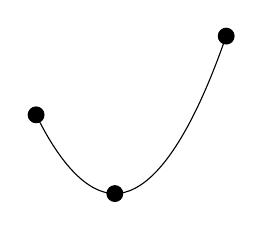
\begin{tikzpicture}
\draw (-1,1) parabola bend (0,0) (1.414,2);
\filldraw (-1,1) circle (.1)
    (0,0) circle (.1)
    (1.414,2) circle (.1);
\end{tikzpicture}
}
\draw (-1,1) parabola 
    bend (0,0) (1.414,2);
\end{fdemo}

\subsection{圖形控制}
\subsubsection{線型和箭頭}
繪圖命令可以設置線型和箭頭參數。
\begin{fdemo}{
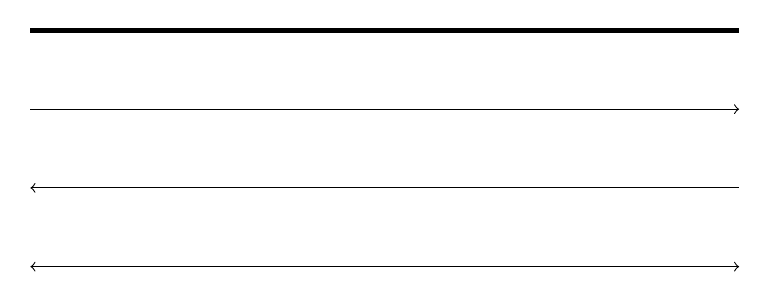
\begin{tikzpicture}
\draw[line width=2pt] (0,3)--(9,3);
\draw[->] (0,2)--(9,2);
\draw[<-] (0,1)--(9,1);
\draw[<->] (0,0)--(9,0);
\end{tikzpicture}
}
\draw[line width=2pt] (0,0)--(9,0);
\draw[->] (0,1)--(9,1);
\draw[<-] (0,2)--(9,2);
\draw[<->] (0,3)--(9,3);
\end{fdemo}

\subsubsection{顏色、填充、陰影}
顏色參數的用法如下。PGF~可以使用~\verb|xcolor|~宏包\citep{Kern_2007}中定義的所有顏色。
\begin{fdemo}{
\begin{tikzpicture}
\draw[red] (0,4)--(9,4);
\draw[green] (0,2)--(9,2);
\draw[blue] (0,0)--(9,0);
\end{tikzpicture}
}
\draw[red] (0,4)--(9,4);
\draw[green] (0,2)--(9,2);
\draw[blue] (0,0)--(9,0);
\end{fdemo}

封閉路徑可以用顏色填充,\verb|\filldraw|~命令可以分別指定邊框色和填充色。
\begin{fdemo}{

\begin{tikzpicture}
\fill[red] (1,1) circle (1);
\filldraw[fill=lightgray,draw=black] 
    (4,1) circle (1);
\end{tikzpicture}
}
\fill[red] (1,1) circle (1);
\filldraw[fill=lightgray,draw=black] 
    (4,1) circle (1);
\end{fdemo}

\verb|\shade|~命令可以產生漸變和光影效果,預設是從上到下,灰色漸變為白色。我們也可以使用其它方向和顏色的漸變。
\begin{code}
\shade (0,0) rectangle (2,2);
\shade[left color=red,right color=orange] (3,0) rectangle (5,2);
\shade[inner color=red,outer color=orange] (6,0) rectangle (8,2);
\shade[ball color=blue] (10,1) circle (1);
\end{code}

\begin{out}

\begin{tikzpicture}
\shade (0,0) rectangle (2,2);
\shade[left color=red,right color=orange] (3,0) rectangle (5,2);
\shade[inner color=red,outer color=orange] (6,0) rectangle (8,2);
\shade[ball color=blue] (10,1) circle (1);
\end{tikzpicture}
\end{out}

\subsubsection{圖形變換}
對圖形對象可以進行平移和旋轉操作,注意如果兩種操作同時進行,它們是有順序的。注意預定義的長度單位在這裡對平移參數失效。
\begin{code}
\draw (0,0) rectangle (2,2);
\draw[xshift=30pt] (0,0) rectangle (2,2);
\draw[xshift=75pt,rotate=45] (0,0) rectangle (2,2);
\end{code}

\begin{out}
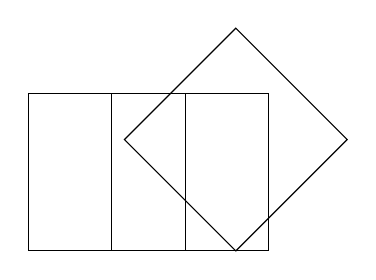
\begin{tikzpicture}
\draw (0,0) rectangle (2,2);
\draw[xshift=30pt] (0,0) rectangle (2,2);
\draw[xshift=75pt,rotate=45] (0,0) rectangle (2,2);
\end{tikzpicture}
\end{out}

\subsection{樣式}
PGF~比~\MP~和~PSTricks~多了一個有趣的概念:樣式(style),它的思路和~HTML~的~CSS~相近。我們可以先定義兩種樣式,
\tikzset{
    myline/.style={line width=2pt},
    myblueline/.style={myline,blue}
}
\begin{code}
\tikzset{
    myline/.style={line width=2pt},
    myblueline/.style={myline,blue}
}
\end{code}

然後就可以在繪圖命令中這樣使用樣式。
\begin{fdemo}{
\begin{tikzpicture}
\draw[myline] (0,2)--(9,2);
\draw[myblueline] (0,0)--(9,0);
\end{tikzpicture}
}
\draw[myline] (0,2)--(9,2);
\draw[myblueline] (0,0)--(9,0);
\end{fdemo}

除了用~\verb|\tikzset|~命令定義樣式,我們也可以在~\verb|tikzpicture|~環境頭部聲明樣式。前者是全局性的,後者則是局部性的。
\begin{code}
\begin{tikzpicture}[
    thickline/.style=2pt,
    bluethickline/.style={thickline,color=blue}
]
...
\end{tikzpicture}
\end{code}

注意在樣式中預定義長度單位有時會失效,所以最好使用絕對單位。

\subsection{流程圖}
\subsubsection{節點}
PGF~中的節點(node)可以是簡單的標籤,也可以有各種形狀的邊框,還可以有各種複雜的屬性。比如下例中的節點樣式:\verb|box|,它的邊框是矩形,有圓角;它有最小寬度、高度、文字和邊框的距離,邊框和填充顏色等屬性。

\begin{code}
\tikzset{
    box/.style={rectangle, rounded corners=6pt, 
        minimum width=50pt, minimum height=20pt, inner sep=6pt, 
        draw=gray,thick, fill=lightgray}
}
\end{code}

除了上述類別屬性,節點還可以有名字、位置等屬性。在下例中,我們先畫了三個有名字的文本框;然後用箭頭把文本框連接起來,注意連接時要引用文本框的名字;接著在箭頭上加了標籤。
\begin{code}
\node[box] (tex) at(0,0) {.tex};  %文本框
\node[box] (dvi) at(10,0) {.dvi}; %文本框
\node[box] (pdf) at(20,0) {.pdf}; %文本框
\draw[->] (tex)--(dvi);           %箭頭
\draw[->] (dvi)--(pdf);           %箭頭
\node at (5,1) {latex};           %標籤
\node at (15,1) {dvipdfmx};       %標籤
\end{code}

\begin{out}
\begin{tikzpicture}
\node[box] (tex) at(0,0) {.tex};
\node[box] (dvi) at(10,0) {.dvi};
\node[box] (pdf) at(20,0) {.pdf};
\draw[->] (tex)--(dvi);
\draw[->] (dvi)--(pdf);
\node at (5,1) {latex};
\node at (15,1) {dvipdfmx};
\end{tikzpicture}
\end{out}

在上例中的節點都使用了絕對位置,PGF~中還可以使用更靈活一點的相對位置。比如在下例中,dvi~節點在~tex~節點右邊~50pt~處(我們前面定義的基本長度單位是~10pt),而~pdf~節點又在~dvi~節點右邊~50pt~處。

箭頭可以換為專門用來連接節點的~\verb|edge|~;標籤也改成相對位置,箭頭上方~5pt~處。
\begin{code}
\node[box] (tex) {.tex};
\node[box,right=5 of tex] (dvi) {.dvi};
\node[box,right=6 of dvi] (pdf) {.pdf};
\path (tex) edge[->]  node[above=.5] {latex} (dvi)
    (dvi) edge[->] node[above=.5] {dvipdfmx} (pdf);
\end{code}

\begin{out}
\begin{tikzpicture}
\node[box] (tex) {.tex};
\node[box,right=5 of tex] (dvi) {.dvi};
\node[box,right=6 of dvi] (pdf) {.pdf};
\path (tex) edge[->]  node[above=.5] {latex} (dvi)
    (dvi) edge[->] node[above=.5] {dvipdfmx} (pdf);
\end{tikzpicture}
\end{out}

\subsubsection{樹}
下面是一棵簡單的樹。我們可以用一個參數控制相鄰節點的距離,預定義長度單位對此參數也會失效。
\begin{code}
\begin{tikzpicture}[sibling distance=80pt]
\node[box] {TeX}
    child {node[box] {Plain\TeX}}
    child {node[box] {\LaTeX}
        child {node[box] {MiKTeX}}
        child {node[box] {TeX Live}}
        child {node[box] {MacTeX}}
    };
\end{tikzpicture}
\end{code}

\begin{out}
\begin{tikzpicture}[sibling distance=80pt]
\node[box] {TeX}
    child {node[box] {Plain\TeX}}
    child {node[box] {\LaTeX}
        child {node[box] {MiKTeX}}
        child {node[box] {TeX Live}}
        child {node[box] {MacTeX}}
    };
\end{tikzpicture}
\end{out}

\bibliographystyle{unsrtnat}
\bibliography{reading}
\newpage


